\documentclass[a4paper,10pt]{article}
\usepackage{listings}
\usepackage{color}
\usepackage{graphicx}

\lstset{language=Java}
\lstset{breaklines=true, numbers=left}
\lstset{tabsize=4}

\definecolor{CommentColor}{rgb}{0,0.5,0} 
\definecolor{KeywordColor}{rgb}{0,0,0.5}

\lstset{commentstyle=\scriptsize\color{CommentColor}\itshape}
\lstset{keywordstyle=\scriptsize\color{KeywordColor}\bfseries}
\lstset{basicstyle=\scriptsize}
\lstset{identifierstyle=\scriptsize}
\lstset{stringstyle=\scriptsize}

% \lstset{basicstyle=\ttfamily}

\definecolor{lightblue}{rgb}{0.7,0.7,1}
\definecolor{lightyellow}{rgb}{1,1,0.5}
\definecolor{lightred}{rgb}{1,0.5,0.5}
\definecolor{lightgreen}{rgb}{0.7,1,0.7}

\newcommand{\src}[1]{\texttt{#1}}

% thanks to http://www.alfredklomp.com/programming/tex/macros/
\long\def\greybox#1#2#3{%
    \newbox\contentbox%
    \newbox\bkgdbox%
    \setbox\contentbox\hbox to \hsize{%
        \vtop{
            \kern\columnsep
            \hbox to \hsize{%
                \kern\columnsep%
                \advance\hsize by -2\columnsep%
                \parbox{0.1\hsize}{\includegraphics[width=\hsize]{#2}}%
                \hspace{0.025\hsize}%
                \advance\hsize by -0.125\hsize%
                \setlength{\textwidth}{\hsize}%
                \vbox{
                    \parskip=\baselineskip
                    \parindent=0bp
                    \parbox[c]{\hsize}{#3}
                }%
                \kern\columnsep%
            }%
            \kern\columnsep%
        }%
    }%
    \setbox\bkgdbox\vbox{
	\color{#1}
        \hrule width  \wd\contentbox %
               height \ht\contentbox %
               depth  \dp\contentbox
	\color{black}
    }%
    \wd\bkgdbox=0bp%
    \vbox{\hbox to \hsize{\box\bkgdbox\box\contentbox}}%
    \vskip\baselineskip%
}

\newcommand{\designbox}[1]{\greybox{lightgreen}{design}{#1}}
\newcommand{\classbox}[1]{\greybox{lightyellow}{class}{#1}}
\newcommand{\warningbox}[1]{\greybox{lightred}{stop}{#1}}
\newcommand{\infobox}[1]{\greybox{lightblue}{info}{#1}}

\title{DockingFrames 1.0.6 - Core}
\author{Benjamin Sigg}

\begin{document}

\maketitle
\tableofcontents
\newpage


\begin{abstract}
 \src{DockingFrames} is an open source Java Swing framework. This project allows to write applications with floating panels, meaning that the user can freely choose where to place the panels.

\src{DockingFrames} is divided into two projects, \src{Core} and \src{Common}. This document only covers \src{Core}, \src{Common} has its own guide.

The goal of this document is to provide any developer with a basic understanding of \src{DockingFrames}. One will not be able to rewrite the project after reading this document, but one will be able to start digging in the source.
\end{abstract}


\section{Notation}
This document uses various notations.

Any element that can be source code (i.e. a class name) and project names are written monospaced like this: \src{java.lang.String}. The package of classes and interfaces is rarely given since almost no name is used twice. The packages can be easily found with the help of the generated api documentation (JavaDoc).

\infobox{Tipps and tricks are listed in boxes.}

\warningbox{Important notes and warnings are listed in boxes like this one.}

\classbox{Implementation details, especially lists of class names, are written in boxes like this.}

\designbox{These boxes explain \textit{why} some thing was designed the way it is. This might either contain some bit of history or an explanation why some akward design is as bad as it first looks.}

\section{Basics}
The basic idea of \src{Core} is to have one object that controlls the framework, one object for each floating panel and one object for each area where a floating panel can be docked.

\classbox{The controller is a \src{DockController}, the floating panels are \src{Dockable}s and the dock-areas are \src{DockStation}s.}

\subsection{Hello World}
Let's start with a simple hello world. This application uses the three basic components, the example consists of valid code and can run:
\begin{lstlisting}
import javax.swing.JFrame;

import bibliothek.gui.DockController;
import bibliothek.gui.dock.DefaultDockable;
import bibliothek.gui.dock.SplitDockStation;
import bibliothek.gui.dock.station.split.SplitDockGrid;

public class HelloWorld {
	public static void main( String[] args ) {
		DockController controller = new DockController();

		SplitDockStation station = new SplitDockStation();
		controller.add( station );
	
		SplitDockGrid grid = new SplitDockGrid();
		grid.addDockable( 0, 0, 2, 1, new DefaultDockable( "N" ) );
		grid.addDockable( 0, 1, 1, 1, new DefaultDockable( "SW" ) );
		grid.addDockable( 1, 1, 1, 1, new DefaultDockable( "SE" ) );
		station.dropTree( grid.toTree() );
	
		JFrame frame = new JFrame();
		frame.add( station.getComponent() );
	
		frame.setDefaultCloseOperation( JFrame.EXIT_ON_CLOSE );
		frame.setBounds( 20, 20, 400, 400 );
		frame.setVisible( true );
	}
}
\end{lstlisting}
What happens here? In line \src{10} a \src{DockController} is created. The controller will handle things like drag and drop. All elements will be in his realm. In line \src{12} a new \src{DockStation} is created and in line \src{13} this station is registered as root station at the \src{DockController}.

Then in line \src{15-19} a few children for \src{station} are generated. To set the layout of those children a \src{SplitDockGrid} is used. \src{SplitDockGrid} takes a few \src{Dockable}s and their position and puts this information into a form that can be understood by \src{SplitDockStation} (line \src{19}). It would be possible to add the \src{Dockable}s directly to the station, but this is the easy way.

In line \src{21} a new frame is created and in line \src{22} our \src{DockStation} is added to the frame.

\infobox{More demonstration applications can be found in the big archive-file of \src{DockingFrames}. Each demonstration concentrates its attention on one feature of the framework.}

\subsection{Dockable}
A \src{Dockable} represents a floating panel, it consists at least of some \src{JComponent} (the panel it represents), some \src{Icon} and some text for a title. Each \src{Dockable} can be dragged by the user and dropped over a \src{DockStation}.

Clients can implement the interface \src{Dockable}, but it is much less painful just to use \src{DefaultDockable}. A \src{DefaultDockable} behaves in many ways like the well known \src{JFrame}: title, icon and panel can be set and replaced at any time.

A small example:
\begin{lstlisting}
DefaultDockable dockable = new DefaultDockable();
dockable.setTitleText( "I'm a JTree" );
Container content = dockable.getContentPane();
content.setLayout( new GridLayout( 1, 1 ) );
content.add( new JScrollPane( new JTree() ) );
\end{lstlisting}

\warningbox{If implementing \src{Dockable}, pay special attention to the api-doc. Some methods have a rather special behavior. It might be a good idea to subclass \src{AbstractDockable} or to copy as much as possible from it.}

\designbox{A careful analysis of \src{Dockable} reveals that there is no way for applications to store their own properties within a \src{Dockable} (unless using a subclass...). There are two reasons for this. First: if only using the default implementation, there is no need for clients to track these properties, store and load them or to delete them once they are no longer used. It is the responsibility of the framework to do so. Second: No special component within the framework or programming technique gets an unfair advantage over others, everything has to be designed in a way that it can work with any new, unknown, crazy other otherwise unexpected kind of \src{Dockable}.}

\subsection{DockStation}
\src{Dockable}s can never fly around for themself, they need a \src{DockStation} as anchor point. The relationship between \src{DockStation} and \src{Dockable} can best be described as parent-child-relationship. A \src{DockStation} can have many children, but a \src{Dockable} only one parent.

There are some classes which are \src{DockStation} and \src{Dockable} at the same time. They allow to build a tree of \src{DockStation}s and \src{Dockable}s. The number of such trees is \textit{not} limited to one.

There are different kind of \src{DockStation}s, each kind has its unique behavior and abilities.
\begin{description}
 \item[StackDockStation] The children are organized like on a \src{JTabbedPane}. Only one child is visible, but another can be made visible by clicking some button.
 \item[SplitDockStation] The children are organized like in a tree of \src{JSplitPane}s. All children are visible and the user can change the (relative) size of the \src{Dockable}s.
 \item[FlapDockStation] Much like \src{StackDockStation} but the one visible child pops up in its own window. This station can also show no \src{Dockable} at all.
 \item[ScreenDockStation] Shows each child in its own window.
\end{description}

Clients can implement new \src{DockStation}s. But be warned that the interface contains many methods and a lot of them require a lot of code. Don't expect to write less than 1000 lines of code.

A small example that builds a \src{StackDockStation}:
\begin{lstlisting}
StackDockStation stack = new StackDockStation();
stack.setTitleText( "Stack" );
stack.drop( new DefaultDockable( "One" ) );
stack.drop( new DefaultDockable( "Two" ) );
\end{lstlisting}
Some observations: \src{StackDockStation} is a \src{Dockable} as well, in line \src{2} the title is set. Two \src{DefaultDockable}s are put onto the station in lines \src{3,4}, the method \src{drop} is available in all \src{DockStation}s.

\warningbox{\src{DockStation}s are the most complex classes within the framework, they are also among the most important classes. It is very uncommon to subclass them or to write new ones. If you think you need to subclass a \src{DockStation}, be sure to have explored all other options.}

\subsection{DockController}
A \src{DockController} manages almost all the interactions between \src{Dockable}s and \src{DockStation}s. A \src{DockController} seldomly does a task by himself, but it always knows how to find an object that can do the task.

There can be more than one \src{DockController} in an application. Each controller has its own realm and there is no interaction between controllers. Most applications will need only one \src{DockController}.

Clients need to register the root of their \src{DockStation}-\src{Dockable}-trees. They can use the method \src{add} of \src{DockController} to do that. All children of the root will automatically be registered as well. If a \src{DockStation} is not registered anywhere, it just does not work properly. For \src{Dockable}s one could say that registration equals visibility. A registered \src{Dockable} can be seen by the user, an unregistered not.

\classbox{\src{DockController} uses other classes to handle tasks. Many of these classes can be observed by listeners. An incomplete list:

\src{DockRegister}: a list of all \src{Dockable}s and \src{DockStation}s.

\src{DockRelocator}: handles drag and drop operations, can create a \src{Remote} to play around without user interaction.

\src{DoubleClickController}: detects double clicks on \src{Dockable}s or on components which represent \src{Dockable}s.

\src{KeyBoardController}: detects \src{KeyEvent}s on \src{Dockable}s or on components which represent \src{Dockable}s.}

\warningbox{Never forget to register the root-\src{DockStation}(s) at the \src{DockController} using the method \src{add}.}

\designbox{Why not just one \src{DockController} implemented as singleton? A singleton would make many interfaces simpler, eliminating all the code where the controller is handed over to even the smallest object. On the other hand there is absolutely no reason to limit oneself to only one object and there are applications which need more than one controller. In the end not using a singleton just gives more flexibility.}

\subsection{DockFrontend}
\src{DockController} only implements the basic functionallity. While this allows developers to add new exciting shiny customized features, it certainly doesn't help those developers which just want to use the framework.

The class \src{DockFrontend} represents a layer before \src{DockController} and adds a set of helpful methods. Especially a ``close''-button and the ability to store and load the layout are a great help. \src{DockFrontend} replaces \src{DockController}, clients should add the root-\src{DockStation}s directly to the frontend, not to the controller. They can use the method \src{addRoot} to do so.

\warningbox{\src{DockFrontend} adds a few nice features but not enough to write an application without even bothering to have a look at \src{DockingFrames}. Developers which can live with not having absolute control over the framework should use \src{Common}. \src{Common} adds all those features which make a docking-framework complete, i.e. a ``minimize''-button}

\designbox{\src{DockFrontend} was written long after \src{DockController}. For the most part it just reuses code that already exists. It would be possible to write two applications with exact the same behavior once with and once without \src{DockFrontend}. The only thing that \src{DockFrontend} adds to the framework is a central hub where all the important features are accessible and a good set of default-values for various properties of the framework.}

\infobox{Use the methods called \src{setDefault...} to set default values for properties which will be used for \src{Dockable}s. I.e. whether \src{Dockable}s are hideable or not.}

\subsubsection{Close-Button}
In order to show the close-button clients need first to register their \src{Dockable}s. The method \src{addDockable} is used for that. Each \src{Dockable} needs a unique identifier that is used internally by \src{DockFrontend}. Later clients can call the method \src{setHideable} to show or to hide the close-button.

By calling the method \src{setShowHideAction} clients can make the buttons invisible for all \src{Dockable}s, note however that the \src{Dockable}s hideable-property is not affected by this method.

If clients want to control whether a \src{Dockable} can be closed, they should add a \src{VetoableDockFrontendListener} to the \src{DockFrontend}. This listener will be informed before a \src{Dockable} is made invisible and allows to cancel the operation.

\designbox{Why is the close-button not part of the very core of the framework? For one because the very core works on abstract levels and should not be made more complex with special cases like this button. There are also different implementations of this button and not all perform the same actions when pressed (this is especially true when using \src{Common}).}

\subsubsection{Storing the layout}
The methods \src{save}, \src{load}, \src{delete} and \src{getSettings} are an easy way to store and load the layout. This mechanism will be explained in detail in another chapter.

\section{Load and Save layouts}
The layout of an application means the position, size and relationships of all the \src{Dockable}s and \src{DockStation}s. To store this layout on a harddrive and later to load it again is a great help for the user, he does not need to setup the layout over and over again.

\src{DockingFrames} distinguishes between local and global layout information. Local information only describes the relationship between one \src{Dockable} and its parent, global information describes whole trees of elements. There are no algorithms which recreate a whole layout from a set containing local information, but there are also no algorithms which can place a \src{Dockable} in the tree using global information. So both kinds of data have their use.

\subsection{Local: DockableProperty}
Every \src{DockStation} can create a \src{DockableProperty}-object for one of its children. This \src{DockableProperty} contains the position and size of one child.

Some \src{DockStation}s are also \src{Dockable}s. Those stations are not only able to create \src{DockableProperties} for their children but their parents can create a property for them. These two properties can be strung together to form a chain describing the position of a grand-child on its grand-parent.

\subsubsection{Creation}
How to create a \src{DockableProperty}? One way is of course just to create new objects using \src{new XYProperty(...)}. The other way is to retreive them from some \src{DockStation}s and \src{Dockable}s:
\begin{lstlisting}
Dockable dockable = ...

DockStation root = DockUtilities.getRoot( dockable );
DockableProperty location = DockUtilities.getPropertyChain( root, dockable );
\end{lstlisting}
In line \src{1} we get some unknown \src{Dockable}. In line \src{3} the \src{DockStation} which is at the top of the tree of stations and \src{Dockable}s is searched. Then in line \src{4} the location of \src{dockable} in respect to \src{root} is determined.

\classbox{There are five \src{DockableProperties} present in the framework.
\begin{description}
 \item[StackDockProperty] for \src{StackDockStation}, contains just the index of the \src{Dockable} in the stack.
 \item[FlapDockProperty] for \src{FlapDockStation}, contains index, size and whether the \src{Dockable} should hold its position when not focused.
 \item[ScreenDockProperty] for \src{ScreenDockStation}, contains the boundaries of a \src{Dockable} on the screen.
 \item[SplitDockProperty] for \src{SplitDockStation}. This deprecated property contains the boundaries of a \src{Dockable} on the station.
 \item[SplitDockPathProperty] also for \src{SplitDockStation}. This new property contains the exact path leading to a \src{Dockable} in the tree that is used internally by the \src{SplitDockStation}.
\end{description}
}

\subsubsection{Usage}
How to apply a \src{DockableProperty}? Every \src{DockStation} has a method \src{drop} that takes a \src{Dockable} and its position. That might look like this:
\begin{lstlisting}
Dockable dockable = ...
DockStation root = ...
DockableProperty location = ...

if( !root.drop( dockable, location )){
  root.drop( dockable );
}
\end{lstlisting}
In lines \src{1-3} some elements that were stored earlier are described. In line \src{5} we try to drop \src{dockable} on \src{root}, if that fails we just drop it somewhere (line \src{6}).

\src{DockableProperty}s are not safe to use. If the tree of stations and \\\src{Dockable}s changes, then an earlier created \src{DockableProperty} might not be consistent anymore. The method \src{drop} of \src{DockStation} checks for consistency and returns \src{false} if a \src{DockableProperty} is no longer valid.

\warningbox{Always check the result of \src{drop}, if it is \src{false} then the operation was canceled by the station because the property is invalid.}

\subsubsection{Storage}
\src{DockableProperty}s can be stored either as byte-stream or in xml-format by a \src{PropertyTransformer}. A set of \src{DockablePropertyFactories} is used by the transformer to store and load properties. The factories for the default properties are always installed. If a developer adds new properties then he should use the method \src{addFactory} to install new factories for them.

\infobox{If using \src{DockFrontend} the method \src{registerFactory} can be used to add a new \src{DockablePropertyFactory}. This factory will then be used by global transformer of the frontent.}

\subsection{Global: DockSituation}
The layout of a whole set of \src{Dockable}s and \src{DockStation}s can be stored with the help of a \src{DockSituation}. A \src{DockSituation} is a set of algorithms that transform the layout information from one format into another, i.e. from the dock-tree (built by stations and \src{Dockable}s) to an xml-file. A \src{DockSituation} uses various factories to transform one format into another.

\subsubsection{Basic Algorithms}
Global layout information comes in four formats:
\begin{description}
 \item[dock-tree format] The set of \src{Dockable}s and \src{DockStation}s as they are seen by the user.
 \item[binary format] A file containing binary data. This file is normally written by a \src{DataOuputStream} and read by a \src{DataInputStream}.
 \item[xml format] A file containing xml. To write and read such a file the class \src{XIO} is used.
 \item[layout-composition format] An intermediate format that consists of a set of \src{DockLayoutComposition}s. These objects are organized in a tree that has the same form as the dock-tree.
\end{description}
To convert one format into another a \src{DockSituation} is used. If converting from \src{a} to \src{b} then a \src{DockSituation} will always first convert \src{a} to \src{layout-composition} and then \src{layout-composition} to \src{b}.

\warningbox{\src{DockSituation} always creates new files or new objects. In its basic form it is not able to reuse existing elements.}

A \src{DockSituation} uses different factories and strategies for these conversions:
\begin{description}
 \item[DockFactory] These factories are responsible to load or store the layout of a single \src{Dockable} or \src{DockStation}. Like \src{DockSituation} they need to support four formats. For one the dock-element they store or read, then binary- and xml-format and finally some object as intermediate formate. They are free to choose any kind of object as intermediate format.
 \item[AdjacentDockFactory] They function the same way as \src{DockFactories} but can be used for arbitrary dock-elements. \src{AdjacentDockFactories} are used to store additional information about elements, that can, but does not have to be, layout information.
 \item[MissingDockFactory] These are used when another factory is missing. The \src{MissingDockFactory} can try to read the xml-format or binary-format and convert it to the intermediate format.
 \item[DockSituationIgnore] This strategy allows a \src{DockSituation} to ignore dock-elements when storing the layout. That can be helpful if i.e. an application has \src{Dockable}s which show only temporary information that will be lost on shutdown anyway.
 \end{description}

A \src{DockSituation} can handle missing factories when reading xml or binary format. It first tries to use a \src{MissingDockFatory} to read the data, if that fails it either throws away the data (for \src{AdjacentDockFactories}) or stores the data in the layout-composition as ``bubble'' in its raw format. These ``bubbles'' can be converted later when the missing factories are found.

\classbox{A \src{DockLayoutComposition} contains a lot of information. First of all a list of children to build the tree. Then a list of \src{DockLayout}s which represent the information from \src{AdjacentDockFactories}. Each \src{DockLayout} contains a unique identifier for the factory and the data generated by the factory. Finally a \src{DockLayoutComposition} contains a \src{DockLayoutInfo} which represents the data of or for a \src{DockFactory}. A \src{DockLayoutInfo} either contains a \src{DockLayout} (the normal case) or some data in xml or binary format. The later case happens if a factory was missing while reading a file, the information gets stored until it can be read later.}

\infobox{The method \src{fillMissing} can be used to read ``bubbles'' in raw format. The method \src{estimateLocations} can be used to build \src{DockableProperties} for the elements. These are the positions were the elements would come to rest if the layout information were converted into a dock-tree.}

\subsubsection{Basic Usage}
How is a \src{DockSituation} utilized in order to load or store the layout of an application?

Each \src{Dockable} and each \src{DockStation} have a method \src{getFactoryID}. This method returns an identifier that has to match the unique identifier that is returned by the method \src{getID} of \src{DockFactory}. So the first step in using a \src{DockSituation} will always be to make sure that for any identifier a matching \src{DockFactory} is available. Clients will call the method \src{add} of \src{DockSituation} to do so.

\infobox{Default factories are installed for \src{DefaultDockable}, \src{SplitDockStation}, \src{StackDockStation} and \src{FlapDockStation}.}

\warningbox{The \src{ScreenDockStationFactory} for \src{ScreenDockStation} is not installed per default. This factory requires a \src{WindowProvider} to create the station, and since this provider cannot be guessed by \src{DockSituation} the factory is missing. Clients have to add \src{ScreenDockStationFactory} manually.}

Afterwards clients just have to call \src{write} or \src{writeXML} to write a set of \src{DockStation}s and their children. Clients can later call \src{read} or \src{readXML} to read the same map of elements. Note that every call to \src{read} or \src{readXML} will create a new set of \src{Dockable}- and \src{DockStation}-objects.

Let't give an example how to write an xml file:
\begin{lstlisting}
try{
	JFrame frame = ...
	DockStation root = ...

	DockSituation situation = new DockSituation();
	situation.add( new ScreenDockStationFactory( frame ) );
	situation.add( new MySpecialFactory() );

	Map<String, DockStation> map = new HashMap<String, DockStation>();
	map.put( "root", root );

	XElement xlayout = new XElement( "layout" );
	situation.writeXML( map, xlayout );

	FileOutputStream out = new FileOutputStream( "layout.xml" );
	XIO.writeUTF( xlayout, out );
	out.close();
}
catch( IOException ex ){
	ex.printStackTrace();
}
\end{lstlisting}
On line \src{2} the main-frame of the application is given and on line \src{3} the applications root \src{DockStation}. The first step is to create a new \src{DockSituation} on line \src{5} and add the missing \src{ScreenDockStationFactory} on line \src{6}. Then other factories that are not part of \src{DockingFrames} but the application itself can be added like on line \src{7}. On lines \src{9, 10} a map with all the root-stations of the application is built up. Then on line \src{12} we prepare for writing in xml-format by creating a \src{XElement}. The situation converts the dock-tree to xml-format in line \src{13}. Finally on lines \src{15-17} the xml-tree is written into a file ``layout.xml''.

The next example shows how reading from binary format can look like:
\begin{lstlisting}
try{
	JFrame frame = ...

	DockSituation situation = new DockSituation();
	situation.add( new ScreenDockStationFactory( frame ) );
	situation.add( new MySpecialFactory() );

	FileInputStream fileStream = new FileInputStream( "layout" );
	DataInputStream in = new DataInputStream( fileStream );

	Map<String, DockStation> map = situation.read( in );

	in.close();

	SplitDockStation station = (SplitDockStation)map.get( "root" );
	frame.add( station.getComponent() );
}
catch( IOException ex ){
	ex.printStackTrace();
}
\end{lstlisting}
What happens here? In line \src{2} the main frame of the application is defined. In lines \src{4-6} a \src{DockSituation} is set up. In lines \src{8, 9} a file is opened. In line \src{11} that file gets read by the \src{DockSituation} and a map that was earlier given to \src{write} is returned. In line \src{15} the fact that \src{map} was earlier given to \src{write} is used to guess that there is a \src{SplitDockStation} with key ``root'' in the map. Finally in line \src{16} that station is put onto the main-frame which now shows the new elements.

\subsubsection{Extended Algorithms}
The major drawback of the basic algorithms is that they always create new \src{Dockable}s and \src{DockStation}s. As a result it is nearly impossible to just change the layout while an application is running, a layout can only be loaded on startup. \src{PredefinedDockSituation} builds upon \src{DockSituation} and extends the algorithms in a way that the can reuse existing dock-elements.

The extended version uses a special \src{DockFactory}, called \src{PreloadFactory}, that is wrapped around the factories providied by the client. Writing does not change much, the \src{PreloadFactory} delegates the work just to the original \src{DockFactory}. Reading is more interesting. The \src{PreloadFactory} forwards the dock-element to reuse to the the original \src{DockFactory} which then updates the layout of the element.

A side effect of this implementation is, that for the basic \src{DockSituation} no factories seem ever to be missing. In fact the issue of missing factories is just moved to the \src{PreloadFactory}. The \src{PreloadFactory} can however store data in its raw format if necessary.

\classbox{A \src{PreloadFactory} uses a \src{PreloadedLayout} as intermediate format. This \src{PreloadedLayout} contains the unique identifier of the original \src{DockFactory} and a \src{DockLayoutInfo}. The \src{DockLayoutInfo} contains either data in raw format or in the intermediate format of the original factory.}

What happens if a \src{PredefinedDockSituation} finds layout information for an element, has all the necessary factories but not the element itself? The default behavior is to ignore the information. However it is possible to use backup-\src{DockFactories}. These backup factories will create new elements if they were missing. They are also used when reading raw format and the original factory is missing. These backup factories are added through \src{addBackup}, they have to use a \src{BackupFactoryData} as intermediate format.

\warningbox{Note that the \src{MissingDockFactory} of \src{DockSituation} is not used for elements that were predefined on writing, because for those elements the \src{PreloadFactory} - which is never missing - was used.}

\designbox{The existence of these two sets of algorithms, basic and extended, lays in the history of \src{DockingFrames}. First the basic algorithms were written. They did their job well for small applications. But when applications began to grow it became evident that their were not sufficient. Instead of rewriting them another layer was added. The division in two sets of algorithms has also the advantage of reduced complexity.

The recovery mechanisms for missing factories were introduced for version 1.0.7. They are not yet satisfying and it is likely that they will be changed again in future versions.}

\subsubsection{Extended Usage}
\src{PredefinedDockSituation} is used in the same way as \src{DockSituation}. The only difference is the possibility to predefine elements. The method \src{put} can be used for that. This method expects a unique identifier for any new element.

An example can look like this:
\begin{lstlisting}
	DockStation rootStation = ...
	Dockable fileTreeDockable = ...
	Dockable contentDockable = ...

	PredefinedDockSituation situation = new PredefinedDockSituation();

	// setup situation {...}

	situation.put( "root", rootStation );
	situation.put( "file-tree", fileTreeDockable );
	situation.put( "content", contentDockable );

	// read or write {...}
\end{lstlisting}
In lines \src{1-3} some \src{DockStation}s and \src{Dockable}s are defined. These are the elements that are always present and need not to be recreated when loading a layout. In line \src{5} a new \src{PredefinedDockSituation} is created. Then the basic setup (adding factories, ...) is done in line \src{7}. In the lines \src{9-11} the predefenied elements are added to the situation. For each of them a unique identifier is choosen. Finally in line \src{13} we can either write or read the layout.

\infobox{Any \src{String} can be used as unique identifier. Small identifiers with no special characters are however much less likely to attract any kind of trouble.}

\subsection{DockFrontend}
\src{DockFrontend} offers storage for local and for global layout information. Clients need to register their \src{Dockable}s through \src{addDockable} if they want access to the full range of storage-features.

\subsubsection{Local}
Whenever \src{hide} is called for a registered \src{Dockable} its local position gets stored. If later \src{show} is called this position is reapplied and the element shows up at the same (or nearly the same) location it was earlier. This local information can also be stored in xml- or binary-format. The methods \src{write}, \src{writeXML}, \src{read} and \src{readXML} will take care of this.

\subsubsection{Global}
\src{DockFrontend} internally uses a \src{PredefinedDockSituation} to store the global layout. All root-\src{DockStation}s and all registered \src{Dockable}s are automatically added to this situation. The global layout can either be stored on disk using the methods \src{write}, \src{writeXML}, \src{read} and \src{readXML} or it can be stored in memory. It is possible to store more than just one layout in memory and allow the user to choose from different layouts. There are methods to interact with the layouts in memory:

\begin{description}
 \item[save] Saves the current layout in memory. Clients can provide a name for the layout or use the name of the last loaded layout.
 \item[load] Loads a layout. The name of the layout is used as key.
 \item[delete] Deletes a layout from memory.
 \item[getSettings] Gets a set of names for the different layouts.
 \item[getCurrentSetting] Gets the name of the layout that is currently loaded, can be \src{null}.
 \item[setCurrentSetting] If there is a layout with the name given to this method than that layout is loaded. Otherwise the current layout gets saved with the new name.
\end{description}

The layouts that are in memory can be stored persistent as well.

\subsubsection{Missing Dockables}
The default behavior of \src{DockFrontend} is to through away information for missing \src{Dockable}s. It is however possible to change that behavior.

If data needs to be stored for a missing \src{Dockable} then \src{DockFrontend} uses an ``empty entry''. Clients can define new empty entries by invoking the method \src{addEmpty}. Existing entries can be removed with \src{removeEmpty}, with \src{listEmpty} all empty entries can be accessed. Once an entry has been marked as ``empty'' it can switch between filled and empty as many times as necessary without loosing its layout information. The \src{DockFrontend} can even store data in raw xml or binary format and convert this data later once an appropriate \src{DockFactory} becomes known.

\infobox{``Empty entries'' are best to be used if a client already knows the identifiers of all the \src{Dockable}s that can eventually be registered at the \src{DockFrontend}.}

Another way is to register backup-\src{DockFactories} by calling the method \src{registerBackupFactory}. These factories will create new \src{Dockable}s which are then automatically registered.

\infobox{A backup-factory is the strongest weapon against missing information. If there is a possibility to use them, use them.}

And finally there is the \src{MissingDockableStrategy} which can be set using \src{setMissingDockableStrategy}. This strategy enables or disables to automatic processes.
\begin{itemize}
 \item It allows to create ``empty entries'' automatically. There are two methods \src{shouldStoreShown} and \src{shouldStoreHidden} which have to check the identifiers and to return \src{true} to allow a new empty entry.
 \item It allows to use new \src{DockFactories} as soon as they become known. Normally \src{DockFrontend} does not change the layout without the explizit command from a client (by invoking \src{setSetting} directly or indirectly). If \src{shouldCreate} returns \src{true} however \src{DockFrontend} will update the layout as soon as enough information is available to do so.
\end{itemize}

\infobox{\src{MissingDockableStrategy} should be used when no information about what is missing is available. It allows to run a ``do whatever is possible''-strategy.}

\warningbox{If a strategy allows to store anything and a client often uses different identifiers for their \src{Dockable}s, then layouts will start to grow and never stop. Don't forget to delete outdated information.}

\classbox{The interface \src{MissingDockableStragey} offers two default implementations: \src{DISCARD\_ALL} and \src{STORE\_ALL}. The first implementation is set as default and allows nothing, the second one allows everything.}

\section{Actions}
All \src{Dockable}s can be associated with some actions. An action normally appears as some kind of button in the title of a \src{Dockable}, they can however appear at other places as well. There are different types of actions, some may behave like a \src{JButton} others like a \src{JCheckBox}, clients can add new types.

\begin{figure}[h]
\centering
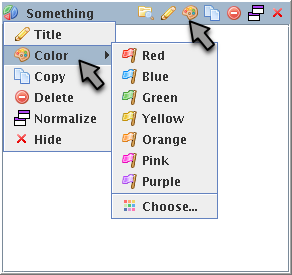
\includegraphics[scale=0.5]{actions}
\caption{A \src{Dockable} with a few \src{DockAction}s in its title and on a popup menu. The action marked by an arrow is the same object just shown in different views.}
\label{fig:actions}
\end{figure}

Actions are represented by the interface \src{DockAction}. Each \src{Dockable} has a list of them represented by a \src{DockActionSource}.

If some component wants to show some actions it firsts asks a \src{Dockable} for its global \src{DockActionSource}. It then asks each \src{DockAction} of that list to create a view that fits to the component. A title will ask for another kind of view than a menu. At any time actions can be added or removed from the \src{DockActionSource} and any component showing actions will react on these events.

\classbox{The interface \src{DockAction} is quite simple. Two methods to install (\src{bind}) and to uninstall (\src{unbind}) the action. One method to create new views (\src{createView}) and one method to trigger an action programatically (\src{trigger}). More useful are the many subclasses and subinterfaces. \src{StandardDockAction} introduces icons, text and tooltip. Five subinterfaces for \src{StandardDockAction} exist and for all of them a default-view is provided.}

\designbox{There are three levels in the design of \src{DockAction} and its subclasses. First there is \src{DockAction} which allows almost any kind of \src{Component} to be used as view. Second there are subinterfaces for the standard tasks, the framework provides views for them. Third are real implementations of the second-level interfaces. Some interfaces are implemented in more than one action for different styles of aplication organization.}

\subsection{Standard Actions}

\section{Titles}
\section{Themes}
\section{Drag and Drop}
\section{Preferences}
\section{Properties}

\end{document}